%%%%%%%%%%%%%%%%%%%%%%%%%%%%%%%%%%%%%
%                                   %
% Compile with XeLaTeX and biber    %
%                                   %
% Questions or comments:            %
%                                   %
% joshua dot mcneill at uga dot edu %
%                                   %
%%%%%%%%%%%%%%%%%%%%%%%%%%%%%%%%%%%%%

\documentclass{beamer}
  % Read in standard preamble (cosmetic stuff)
  %%%%%%%%%%%%%%%%%%%%%%%%%%%%%%%%%%%%%%%%%%%%%%%%%%%%%%%%%%%%%%%%
% This is a standard preamble used in for all slide documents. %
% It basically contains cosmetic settings.                     %
%                                                              %
% Joshua McNeill                                               %
% joshua dot mcneill at uga dot edu                            %
%%%%%%%%%%%%%%%%%%%%%%%%%%%%%%%%%%%%%%%%%%%%%%%%%%%%%%%%%%%%%%%%

% Beamer settings
% \usetheme{Berkeley}
\usetheme{CambridgeUS}
% \usecolortheme{dove}
% \usecolortheme{rose}
\usecolortheme{seagull}
\usefonttheme{professionalfonts}
\usefonttheme{serif}
\setbeamertemplate{bibliography item}{}

% Packages and settings
\usepackage{fontspec}
  \setmainfont{Charis SIL}
\usepackage{hyperref}
  \hypersetup{colorlinks=true,
              allcolors=blue}
\usepackage{graphicx}
  \graphicspath{{../../figures/}}
\usepackage[normalem]{ulem}
\usepackage{enumerate}

% Document information
\author{M. McNeill}
\title[FREN2001]{Français 2001}
\institute{\url{joshua.mcneill@uga.edu}}
\date{}

%% Custom commands
% Lexical items
\newcommand{\lexi}[1]{\textit{#1}}
% Gloss
\newcommand{\gloss}[1]{`#1'}
\newcommand{\tinygloss}[1]{{\tiny`#1'}}
% Orthographic representations
\newcommand{\orth}[1]{$\langle$#1$\rangle$}
% Utterances (pragmatics)
\newcommand{\uttr}[1]{`#1'}
% Sentences (pragmatics)
\newcommand{\sent}[1]{\textit{#1}}
% Base dir for definitions
\newcommand{\defs}{../definitions}


  % Document information
  \subtitle[Variation and Varieties]{Introduction to Language Variation and Language Varieties}

  %% Custom commands
  % Subsection/frame titles
  \newcommand{\suboneone}{What are we looking at?}
  \newcommand{\subtwoone}{What do we mean by ``variety''?}
  \newcommand{\subtwotwo}{Dialects}
  \newcommand{\subtwothree}{Sociolects and registers}
  \newcommand{\subtwofour}{Idiolects and styles}
  \newcommand{\subtwofive}{Jargon and slang}
  \newcommand{\subtwosix}{Standards}

\begin{document}
  % Read in the standard intro slides (title page and table of contents)
  %%%%%%%%%%%%%%%%%%%%%%%%%%%%%%%%%%%%%%%%%%%%%%%%%%%%%%%%%%%%%%%%
% This is a standard set of intro slides used in for all slide %
% documents. It basically contains the title page and table of %
% contents.                                                    %
%                                                              %
% Joshua McNeill                                               %
% joshua dot mcneill at uga dot edu                            %
%%%%%%%%%%%%%%%%%%%%%%%%%%%%%%%%%%%%%%%%%%%%%%%%%%%%%%%%%%%%%%%%

\begin{frame}
  \titlepage
  \tiny{Office: % Basically a variable for office hours location
Gilbert 121\\
        Office hours: % Basically a variable for office hours
 lundi, mercredi, vendredi 10:10--11:10
}
\end{frame}

\begin{frame}
  \tableofcontents[hideallsubsections]
\end{frame}

\AtBeginSection[]{
  \begin{frame}
    \tableofcontents[currentsection,
                     hideallsubsections]
  \end{frame}
}


  \section{Intro to Variation}
    \subsection{\suboneone}
      \begin{frame}{\suboneone}
        \begin{block}{Are there differences between these?}
          \begin{tabular}{r l @{ vs } l}
            1)  & English                                       & Japanese                            \\
            2)  & English in the UK                             & English in the US                   \\
            3)  & English in Georgia                            & English in New Jersey               \\
            4)  & English in Athens                             & English in rural Georgia            \\
            5)  & \multicolumn{2}{l}{English of different communities in Athens}                      \\
            6)  & \multicolumn{2}{l}{English of different individuals within one} \\
                & \multicolumn{2}{l}{community in Athens} \\
            7)  & \multicolumn{2}{l}{Your English in different contexts}
          \end{tabular}
        \end{block}
      \end{frame}

      \begin{frame}{\suboneone}
        \begin{alertblock}{Language variation}
          % Language variation
That part of sociolinguistics that deals with how language varies between communities, between individuals, and within individuals

        \end{alertblock}
        \begin{alertblock}{Sociolinguistics}
          % Sociolinguistics
The study of how language interacts with society and culture

        \end{alertblock}
      \end{frame}

  \section{Language Varieties}
    \subsection{\subtwoone}
      \begin{frame}{\subtwoone}
        \begin{alertblock}{Variety}
          % Variety
Any systematic or systematic-like form of language

        \end{alertblock}
        \begin{block}{Types of varieties}
          Socio-political varieties (i.e., systematic-like)
          \begin{itemize}
            \item Languages % (English vs French)
            \item Dialects % (Appalachian English vs New Yor English)
            \item Sociolects % (Working-class English vs Upper-class English)
            \item Registers % (Newscaster English vs Infant Directed Speech)
          \end{itemize}
          Real systems
          \begin{itemize}
            \item Idiolects
            \item Styles
          \end{itemize}
        \end{block}
      \end{frame}

      \begin{frame}{\subtwoone}
        \begin{block}{Dimensions of variation}
          \begin{itemize}
            \item Lexical variation
            \item Grammatical variation
            \begin{itemize}
              \item i.e., Syntax, morphology, phonology
              \item \alert{Accent}: % Accent
The phonology associated with a variety

            \end{itemize}
          \end{itemize}
        \end{block}
      \end{frame}

    \subsection{\subtwotwo}
      \begin{frame}[t]{\subtwotwo}
        \begin{definition}
          % Dialect
A geographically defined variety

        \end{definition}
        \only<1>{
          \begin{columns}
            \column{0.5\linewidth}
            \begin{alertblock}{}
              This is not a disparaging term in linguistics
            \end{alertblock}
            \begin{example}
              Appalachian English vs New York English
            \end{example}
            \column{0.5\linewidth}
            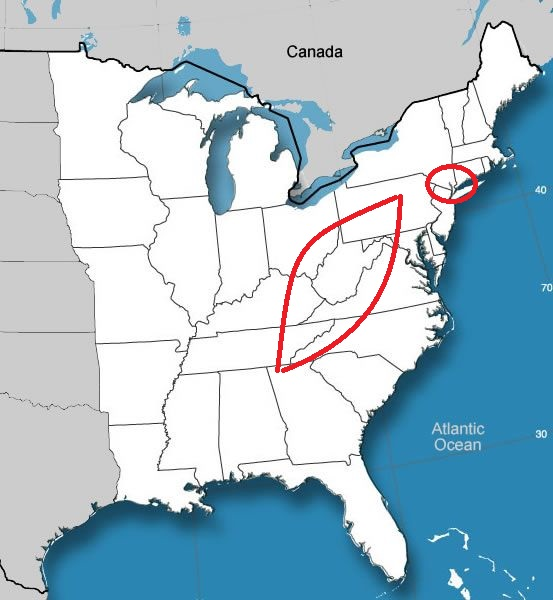
\includegraphics[scale=0.25]{appalachia_new_york.jpg}
          \end{columns}
        }
        \only<2-4>{
          \begin{columns}
            \column{0.5\linewidth}
              \begin{minipage}[t][0.6\textheight]{\linewidth}
                \only<2>{
                  \begin{alertblock}{Speech community}
                    % Speech community
A geographically defined community that shares ways of speaking as well as evaluations for those ways of speaking
 % \parencite{labov_social_2006}
                  \end{alertblock}
                }
                \only<3>{
                  \begin{block}{Extra-linguistic factors that divide up speech communities}
                    \begin{itemize}
                      \item Socioeconomic status
                      \item Age
                      \item Gender
                      \item Ethnicity
                    \end{itemize}
                  \end{block}
                }
                \only<4>{
                  \begin{block}{Not the only conceptualization of community}
                    Speech communities work well for large demographically-driven surveys
                  \end{block}
                }
              \end{minipage}
            \column{0.5\linewidth}
              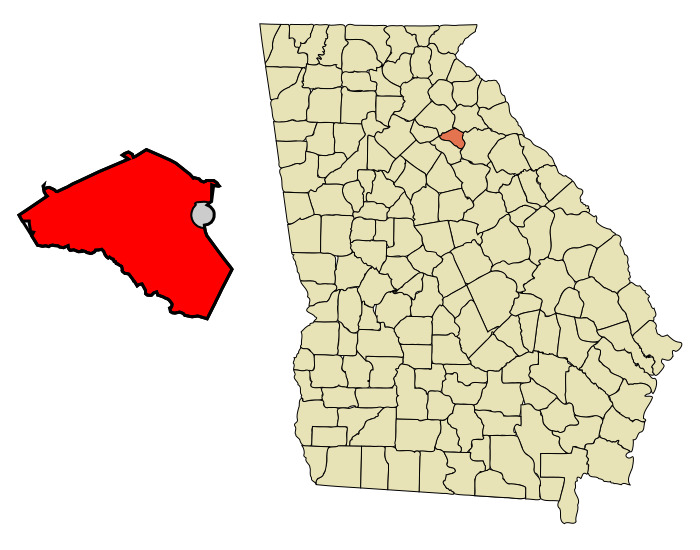
\includegraphics[scale=0.2]{athens.jpg}
          \end{columns}
        }
        \only<5->{
          \begin{block}{How do we tell the difference between dialects and languages?}
            \uncover<6->{
              Mutual intelligibility?
              \begin{itemize}
                \item Difficult to measure % Use video of Jamaican Creole that they can understand parts of
              \end{itemize}
            }
          \end{block}
        }
      \end{frame}

      % "Variety" is generic term: any systematic or systematic-like form of language
        % Dialects
          % What makes languages and dialects different?
            % Mutual intelligibility, however:
              % Measuring it is difficult in the first place
              % Swedes and Norwegians can normally understand each other but speak different "languages"
              % People from different parts of China often can't understand each other but speak different "dialects"
              % Dialect continuums confuse the matter further
                % Define
                % At the Germany-Netherlands border, the Dutch and German speakers can often understand each other, even though speakers of those languages who don't live at the border often can't
            % What really makes languages and dialects different is that speakers consider them to be different
              % They are socio-political constructs
        % Sociolects and registers
          % Where dialects are geographically defined varieties ->
            % Sociolects defined by social class, economic class, or ethnicity more generally
            % Registers defined by activity
        % Idiolects and styles
          % Which utterance would you use to greet the Queen of England?
            % One is appropriate for the context, one is not
          % Definintions: styles first, idiolects next (repertoire of styles)
            % What counts as context? Same as in pragmatics: situational and social
          % Style shifting
            % Define
            % This typically happens subconsciously
        % Jargon and slang
          % Where do these fit in?
          % Both deal purely with lexical expressions
          % Define jargon
            % Useful in style shifting: employ it to sound in-the-know, avoid it to make yourself understandable to others
          % Slang is not well-defined in linguistics
            % Try to define it anyway
            % Useful in style shifting: marks one as being part of a group, in-the-know, and excludes others
        % Standards
          % No variety is superior to another: they're all rule-governed and equally logical
          % However, there are standard varieties
            % Define
            % Double negation example:
              % Used in Chaucer (1) but not considered standard today
              % Point is that the standard is structurally arbitrary
          % Desire to speak the standard for the prestige leads to hypercorrection
            % Use pronoun case in coordinate subjects and objects to demonstrate (3-7)
          % Standards for whole countries often given names:
            % US: Standard American English (SAE)
            % UK: Received Pronunciation (RP)
          % Non-standard varieties are not substandard
            % Maybe show example of reflexive pronoun construction in standard vs non-standard for discussion
            % Being able to use both is advantageous, actually
              % Covert prestige

    \subsection{}
      \begin{frame}{}
        \begin{block}{Try these}
          % \textcite{dawson_language_2016}, chapter 9 exercise 15
        \end{block}
      \end{frame}

      \begin{frame}{References}
        % \printbibliography
      \end{frame}
\end{document}
